\chapter{Minors' Lifestyle Analysis: classificazione} %\label{1cap:spinta_laterale}

% \begin{preamble}
% {\em In questo capitolo conclusivo si cercherà di proporre una procedura di autorizzazione armonica e collegata a quanto emerso nello studio della geotermia a bassa entalpia. Non saranno quindi presi in considerazione le perforazioni geotermiche di profondità, perché esulano dallo scopo del testo e la loro autorizzazione deve essere esaminata caso per caso, mentre le sonde orizzontali e le fondazioni energetiche, pur rientrando nella categoria saranno tralasciate, perché le prime hanno un impatto ambientale trascurabile e sono già regolamentate negli scavi e ripristini per la posa di reti ed impianti e le seconde invece richiedono una progettazione termica/strutturale specialistica.

% Per i sistemi a circuito aperto e chiuso si consiglieranno allora i compiti e le procedure che l'ente di controllo dovrebbe svolgere per concedere l'autorizzazione e la vigilanza degli impianti geotermici e la documentazione che la potenziale committenza dovrebbe fornire per descrivere l'impianto e per mitigare l'impatto ambientale.

% Infine si riporteranno alcuni utili consigli che possono essere prescritti dall'ente di controllo e seguiti dal committente in fase di progettazione, per ridurre l'impatto ambientale da un lato e risparmiare sui costi di perforazione e gestione dall'altro.}
% \end{preamble}

La classificazione è stata condotta con l'obiettivo di sviluppare modelli predittivi in grado di stimare la qualità della dieta dei minorenni sulla base delle loro abitudini di vita e degli altri attributi presenti nel dataset. Il processo ha incluso un'analisi esplorativa approfondita, la gestione dello sbilanciamento delle classi tramite campionamento, l'applicazioni di diversi algoritmi di machine learning (ottimizzati tramite Grid Search) e, infine, l'integrazione di tecniche di Ensemble Learning per tentare di migliorare ulteriormente le prestazioni e la robustezza della classificazione.

\section{Selezione delle feature e pulizia del dataset}

Prima di procedere con le fasi di addestramento e ottimizzazione dei modelli, è stata effettuata un'attenta analisi preliminare degli attributi presenti nel dataset, che ha portato all'eliminazione di un sottoinsieme di colonne non rilevanti o potenzialmente distorsive per il task predittivo:

\begin{itemize}
    \item \textbf{\texttt{user\_id}}: Identificativo univoco dell'utente; trattandosi di un codice seriale privo di valore numerico o semantico, la sua inclusione avrebbe introdotto un rumore casuale non generalizzabile.
    \item \textbf{\texttt{app\_name}}: Nome dell'applicazione, caratterizzato da un valore costante o non informativo ai fini della predizione comportamentale della dieta.
    \item \textbf{\texttt{education\_level}}: Livello di istruzione, escluso in quanto non correlato o non significativo per il target demografico dei minorenni considerato nel perimetro d'analisi.
    \item \textbf{\texttt{last\_login\_date}}: Timestamp relativo all'ultimo accesso, variabile temporale priva di utilità predittiva diretta per la valutazione della qualità della dieta.
    \item \textbf{\texttt{subscription\_status}} e \textbf{\texttt{uses\_premium\_features}}: Attributi di natura commerciale e amministrativa legati all'account dell'utente, totalmente slegati dalle abitudini alimentari e dallo stile di vita.
    \item \textbf{\texttt{content\_type\_preference}} e \textbf{\texttt{preferred\_content\_theme}}: Preferenze sui contenuti multimediali fruiti, ritenute troppo frammentate e prive di una correlazione diretta con il comportamento nutrizionale.
    \item \textbf{\texttt{privacy\_setting\_level}}: Livello di impostazione della privacy, variabile amministrativa irrilevante per la modellazione del target nutrizionale.
    \item \textbf{\texttt{income\_level}}: Livello di reddito, escluso per evitare distorsioni o stime non attendibili, trattandosi di un campione focalizzato sui minorenni dove tale dato risulta spesso stimato o non direttamente incidente sulle abitudini quotidiane rilevate.
    \item \textbf{\texttt{perceived\_stress\_score}}: Punteggio di stress percepito, rimosso in quanto presentava criticità di coerenza o valori non uniformi all'interno della distribuzione complessiva del campione.
\end{itemize}

L'esclusione di queste variabili ha permesso di alleggerire la dimensionalità dello spazio delle feature, focalizzando l'attenzione esclusivamente sugli attributi comportamentali e sullo stile di vita realmente incidenti sul benessere dei soggetti.

\section{Preprocessing del dataset}

Per affrontare il problema dello sbilanciamento delle classi nella variabile target \textit{diet\_quality} (vedi Figura \ref{fig:distribuzione_iniziale}), è stata adottata una combinazione di tecniche di oversampling e undersampling. L'obiettivo era riequilibrare la distribuzione dei campioni per ciascuna classe, fissando il target a 20.000 elementi per categoria, data l'ampia numerosità complessiva del dataset. Questa procedura è stata applicata esclusivamente al dataset di training, preservando il dataset di test per una valutazione finale non influenzata.

\subsection{Bilanciamento del dataset}

Per aumentare il numero di campioni delle classi minoritarie della variabile target \textit{diet\_quality}, è stata utilizzata la tecnica \textit{SMOTE} (Synthetic Minority Over-sampling Technique). Questa tecnica genera nuovi campioni sintetici interpolando tra i campioni esistenti, mantenendo inalterata la distribuzione delle feature. L'intervento è stato combinato con tecniche di sottocampionamento sulla classe maggioritaria per riportare ciascuna categoria a una numerosità bilanciata di riferimento, applicando il processo esclusivamente sul dataset di training per preservare l'integrità del test set.

Per ridurre il numero di campioni delle classi maggioritarie della variabile target \textit{diet\_quality} fino a raggiungere la soglia di bilanciamento stabilita, è stata utilizzata la tecnica di \textit{undersampling} basata sulla clusterizzazione (\textit{ClusterCentroids}). Questo metodo identifica i cluster rappresentativi dei dati originali e seleziona i campioni centrali di ciascun cluster, mantenendo intatta la distribuzione delle feature.

\begin{figure}[H]
    \centering
    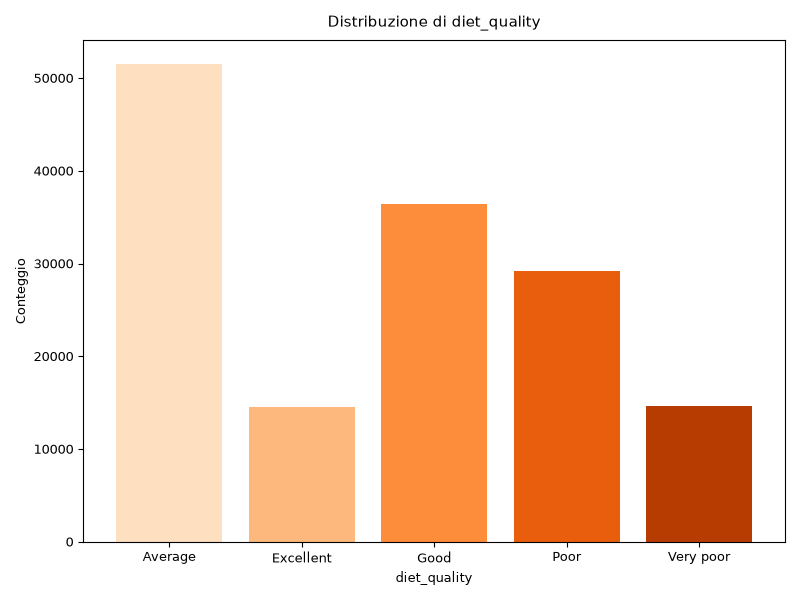
\includegraphics[width=0.8\textwidth]{classificazione/images/distribuzione_diet_quality.png}
    \caption{Distribuzione di diet\_quality prima di applicare le tecniche di sampling}
    \label{fig:distribuzione_iniziale}
\end{figure}

\subsection{Dataset Finale}

Dopo l'applicazione di entrambe le tecniche, il dataset di training bilanciato presenta esattamente 20.000 campioni per ciascuna classe della variabile target \textit{diet\_quality}. Questo dataset è stato salvato in un file CSV per l'addestramento dei modelli, insieme al dataset di test non bilanciato. In Figura \ref{fig:distribuzione_bilanciata} è possibile vedere il risultato della distribuzione dei campioni dopo il processo di bilanciamento.

\begin{figure}[H]
    \centering
    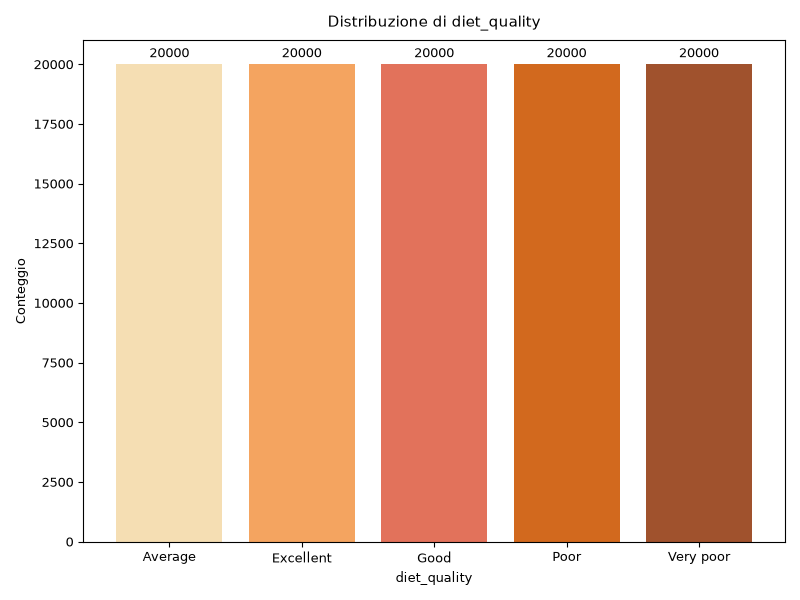
\includegraphics[width=0.8\textwidth]{classificazione/images/distribuzione_diet_quality_bilanciato.png}
    \caption{Distribuzione di diet\_quality dopo il sampling}
    \label{fig:distribuzione_bilanciata}
\end{figure}

\subsection{Analisi della distribuzione degli attributi}

Al termine delle operazioni di oversampling e undersampling, è stata verificata la coerenza della distribuzione degli attributi nel dataset bilanciato. Per questo scopo è stata calcolata e visualizzata la matrice di correlazione delle feature. La matrice di correlazione fornisce una rappresentazione delle relazioni lineari tra le variabili, evidenziando eventuali cambiamenti nella struttura dei dati causati dalle operazioni di bilanciamento. In Figura \ref{fig:correlazione_bilanciata} è possibile vedere la matrice ottenuta dopo le operazioni di sampling.

\begin{figure}[H]
    \centering
    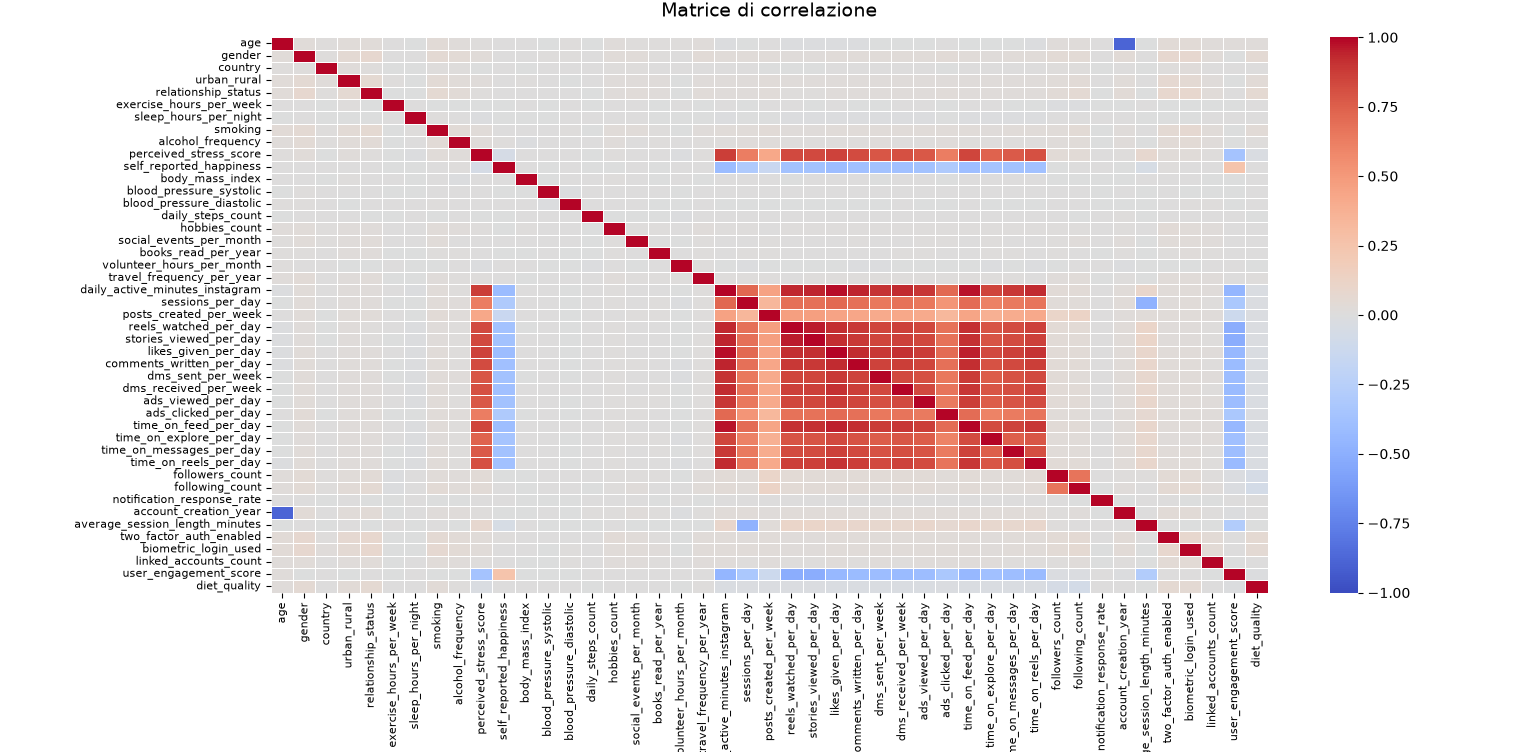
\includegraphics[width=0.9\textwidth]{classificazione/images/matrice_correlazione_bilanciato.png}
    \caption{Matrice di correlazione dopo le operazioni di sampling}
    \label{fig:correlazione_bilanciata}
\end{figure}

L'analisi della matrice di correlazione ha confermato che la distribuzione degli attributi nel dataset bilanciato è rimasta coerente con quella originale. Non sono emerse correlazioni spuriamente elevate o relazioni alterate, a conferma che il bilanciamento delle classi non ha compromesso l'integrità del dataset.

\section{Scenari di Classificazione}

Nel procedere con la classificazione della variabile target \textit{diet\_quality}, l'impostazione degli scenari predittivi è stata guidata dai risultati emersi dall'analisi esplorativa e dalla matrice di correlazione. Al fine di valutare l'impatto degli attributi sul modello e impostare correttamente il task, sono state fatte le seguenti considerazioni metodologiche:

\begin{enumerate}
    \item \textbf{Assenza di attributi derivati (Data Leakage)}: A differenza di altri contesti di studio (in cui figurano attributi continui da cui deriva direttamente e matematicamente la classe target), nel nostro dataset non sono presenti variabili che anticipino deterministicamente la \textit{diet\_quality}. Di conseguenza, non è stato necessario escludere a priori alcuna feature per rischio di \textit{bias} o ridondanza informativa. Rimuovere ulteriori variabili in questa fase avrebbe compromesso l'integrità dell'analisi, impedendo ai modelli di apprendere dai reali pattern comportamentali.
    
    \item \textbf{Inclusione totale delle feature comportamentali}: Dall'analisi della matrice di correlazione (Figura \ref{fig:correlazione_bilanciata}), nessuna variabile è risultata singolarmente ed eccezionalmente correlata con la variabile target. Per questo motivo, si è scelto di non frammentare l'addestramento in scenari multipli per esclusione (es. rimuovendo attributi dominanti per valutarne l'assenza), ma di configurare un \textbf{unico scenario di classificazione completo}. L'obiettivo di questo approccio è fornire in input agli algoritmi l'intero spettro delle variabili (quali ore di sonno, attività fisica, uso dei social) per permettere ai modelli di tentare di individuare relazioni non lineari latenti e sinergie complesse tra gli attributi.
\end{enumerate}

\section{Processo di Classificazione}

Il processo di classificazione è stato applicato allo scenario completo precedentemente descritto, seguendo un approccio strutturato per garantire una valutazione oggettiva. I passi principali hanno incluso l'addestramento dei modelli base, la successiva ottimizzazione dei parametri e l'integrazione finale attraverso tecniche di ensemble learning.
Gli algoritmi di machine learning selezionati per la classificazione della qualità della dieta sono:

\begin{itemize}
    \item \textbf{Random Forest}
    \item \textbf{K-Nearest Neighbors}
    \item \textbf{Decision Tree}
    \item \textbf{Naive Bayes}
    \item \textbf{AdaBoost Classifier}
    \item \textbf{Gradient Boosting Classifier}
\end{itemize}

Si è proceduto in prima istanza addestrando i modelli con i parametri di default, al fine di stabilire una \textit{baseline} prestazionale per valutare i successivi miglioramenti derivanti da approcci più sofisticati. I modelli sono stati addestrati sul dataset bilanciato e testati sul test set originale. I risultati preliminari, espressi in termini di accuratezza media (\textit{Mean Accuracy}), sono riportati di seguito:

\begin{table}[H]
    \centering
    \begin{tabular}{|c|l|c|}
    \hline
    \textbf{Index} & \textbf{Model} & \textbf{Mean Accuracy} \\ \hline
    0 & Random Forest & 0.1967 \\ \hline
    1 & K-Nearest Neighbors & 0.2158 \\ \hline
    2 & Decision Tree & 0.1893 \\ \hline
    3 & Naive Bayes & 0.1707 \\ \hline
    4 & AdaBoost Classifier & 0.2154 \\ \hline
    5 & Gradient Boosting Classifier & 0.2105 \\ \hline
    \end{tabular}
    \caption{Confronto delle performance dei modelli base: accuratezza media calcolata sul test set}
    \label{tab:modelli_base}
\end{table}

Come si evince dai risultati in Tabella \ref{tab:modelli_base}, le prestazioni iniziali si attestano mediamente intorno al 20\%. Questo valore, pur apparendo esiguo, è coerente con la complessità intrinseca del dataset e conferma le difficoltà predittive già anticipate dall'analisi esplorativa della matrice di correlazione.

\subsection{Ottimizzazione dei Modelli}

Al fine di migliorare le prestazioni ottenute con le configurazioni di base, è stata applicata la tecnica della \textit{Grid Search} combinata con una \textit{5-fold cross-validation}. Questo approccio ha permesso di testare diverse combinazioni di iperparametri per individuare la configurazione ottimale per i modelli ritenuti più promettenti, ovvero Random Forest e K-Nearest Neighbors. 

Per garantire l'efficienza computazionale su un dataset di grandi dimensioni, la ricerca degli iperparametri è stata condotta su un campione stratificato del training set bilanciato. I modelli ottimizzati sono stati successivamente riaddestrati sull'intero set di addestramento e valutati sul test set originale. I risultati post-ottimizzazione sono riportati nella Tabella \ref{tab:modelli_ottimizzati}.

\begin{table}[H]
    \centering
    \begin{tabular}{|c|l|c|}
    \hline
    \textbf{Index} & \textbf{Model} & \textbf{Ottimizzato Mean Accuracy} \\ \hline
    0 & Random Forest & 0.2011 \\ \hline
    1 & K-Nearest Neighbors & 0.1875 \\ \hline
    \end{tabular}
    \caption{Confronto delle performance dei modelli a seguito dell'ottimizzazione tramite Grid Search}
    \label{tab:modelli_ottimizzati}
\end{table}

Come si può osservare, l'ottimizzazione degli iperparametri ha prodotto lievi variazioni prestazionali ma non ha portato a un incremento sostanziale dell'accuratezza, confermando la rigidità del task predittivo. Per tentare di superare questo limite strutturale, il passo metodologico successivo è consistito nell'applicazione di tecniche di Ensemble Learning.

\section{Competenze del committente}
Realizzare un sistema geotermico è attualmente oneroso e richiede una progettazione specialistica che pochi installatori possono assicurare o certificare. Il costo iniziale poi è più elevato degli impianti tradizionali e richiede la redazione di relazioni tecniche e idrogeologiche che interessano molteplici figure professionali, sia per il dimensionamento dell'impianto, sia per ottenere la concessione.

\'E bene esserne consapevoli e ricorrere a questo tipo di soluzione per impianti di una certa importanza e che possano servire più utenze. In questo modo si possono ridurre i costi ottimizzando le perforazioni e la gestione del sottosuolo e si possono prevedere analisi e progettazioni più dettagliate.

Inoltre un dimensionamento ottimale dei fabbisogni termici può contribuire a ridurre gli interventi sul terreno che rappresentano la parte più significativa del costo dell'impianto. Vale la pena poi considerare nell'analisi costi/benefici, l'installazione di un sistema ibrido per coprire il carico di picco, se quest'ultimo si raggiunge per poche ore all'anno e far coprire al sistema geotermico il restante \numprint[\%]{90} dell'energia termica richiesta.

Seguendo ed integrando quanto proposto da \cite{anipa}, la committenza per ottenere l'autorizzazione alla realizzazione degli impianti geotermici, dovrà produrre una:
\begin{itemize}
\item domanda da presentare agli organi competenti;
\item relazione idrogeologica preliminare;
%\item competenza della direzione lavori;
\item relazione idrogeologica finale.
\end{itemize}

Di seguito verranno schematizzati i contenuti base di queste domande e relazioni, suddividendole per tipo di impianto ed elencando le competenze della direzione lavori. Ovviamente gli enti di controllo richiederanno maggiori richieste, prescrizioni ed integrazioni a quanto sommariamente elencato. Qui si vuole solo fornire un quadro sintetico e generale, con evidenziate le richieste utili per richiedere ed agevolare l'autorizzazione.

\newpage
\section{Domanda e relazione tecnica preliminare}
La domanda per i due sistemi comprenderà:
\begin{itemize}
\item dati anagrafici del richiedente;
\item dati del progettista e della Direzione Lavori (se differente);
\item dati indicativi della ditta e/o ditte (con eventuali certificazioni);
\item dati significativi dell'impianto (perforazione e installazione);
\item dati indicativi sull'ubicazione dell'impianto.
\end{itemize}

Dovranno poi essere allegati:
\begin{itemize}
\item relazione tecnica di progetto;
\item corografia ubicativa 1:\numprint[]{25000} e planimetria catastale 1:\numprint[]{2000}; 
\end{itemize}

\begin{table}[ht!]%\footnotesize
		\centering
{\footnotesize
	\begin{tabular}{lll}
	\toprule
{\bf componenti}		&	{\bf valore} 		&	{\bf unità di misura} 	\\
	\midrule
materiale organico	(possibilità di sedimentazione)	&	nessuna		&	-	\\
valore di pH		&	$6,5 \div 9$		&	-	\\
conduttività elettrica		&	$50 \div \numprint[]{1000}$		&	$ \mu \: \mathrm{S} \: \mathrm{cm^{-1}}$	\\
cloruro		&	$< 300$		&	$\mathrm{mg} \: \mathrm{\ell^{-1}}$	\\
ferro e manganese		&	$<1$		&	$\mathrm{mg} \: \mathrm{\ell^{-1}}$	\\
solfato		&	$<2$		&	$\mathrm{mg} \: \mathrm{\ell^{-1}}$ \\
contenuto di O\ped{2}		&	$<2$		&	$\mathrm{mg} \: \mathrm{\ell^{-1}}$	\\
cloro		&	$0\div5$		&	$\mathrm{mg} \: \mathrm{\ell^{-1}}$	\\
nitrato		&	$0\div100$	&	$\mathrm{mg} \: \mathrm{\ell^{-1}}$	\\
	\bottomrule
	\end{tabular}%
}

\caption{Requisiti dell'acqua estratta per gli impianti open loop \citep{uni_15450}}
\label{2tab:valori_richiesti_pdc}
\end{table}

\subsection{Per sistemi open loop}
La relazione tecnica comprenderà:
\begin{description}
\item[$\blacktriangleright$] Dati tecnici
\begin{itemize}
\item potenza dell'impianto ($\mathrm{kW\ped{t}}$);
\item fabbisogno termico mensile, con carico medio e di picco;
\item portata necessaria ($\mathrm{m\ap{3}s\ap{-1}}$);
\item $\Delta \mathrm{T}$ (K o $\celsius$);
\item dotazioni di sicurezza e controllo.
\end{itemize}
\item[$\blacktriangleright$] Dati idrogeologici
\begin{itemize}
\item controllo dei vincoli esistenti nell'area di indagine;
\item inquadramento geologico;
\item idrogeologia del sottosuolo (caratteristiche dell'acquifero, permeabilità e direzione di flusso);
\item censimento dei pozzi esistenti nell'area e di altre perforazioni:
\item analisi qualitativa dell'acqua prelevata e restituita alla falda.
\end{itemize}
\item[$\blacktriangleright$] Progetto
\begin{itemize}
\item schema di progetto per la costruzione dei pozzi, con particolare riferimento a diametri e materiali di filtri e rivestimento;
\item descrizione sulle metodologie previste per eseguire a regola d'arte la cementazione del foro;
\item valutazioni sulle possibili conseguenze relative al prelievo dell'acqua e sulla reimmissione, indicando il $\Delta T$ previsto a breve e a lungo termine (il massimo ammesso è di \numprint[\tccelsius]{5}) e la compatibilità ambientale dello scarico nel corpo recipiente.
\end{itemize}
\end{description}

\subsection{Per sistemi closed loop}
La relazione tecnica comprenderà:
\begin{description}
\item[$\blacktriangleright$] Dati tecnici
\begin{itemize}
\item potenza dell'impianto (kW\ped{t});
\item fabbisogno termico mensile, con carico medio e di picco;
\item fluidi, additivi e anticongelanti che verranno utilizzati;
\item $\Delta \mathrm{T}$ (K o $\celsius$);
\item dotazioni di sicurezza e controllo.
\end{itemize}
\item[$\blacktriangleright$] Dati idrogeologici
\begin{itemize}
\item controllo dei vincoli esistenti nell'area di indagine;
\item inquadramento geologico;
\item idrogeologia del sottosuolo (caratteristiche dell'acquifero o degli acquiferi attraversati, permeabilità e direzione di flusso);
\item censimento dei pozzi esistenti nell'area e di altre perforazioni.
\end{itemize}
\item[$\blacktriangleright$] Progetto
\begin{itemize}
\item schema di progetto per la costruzione della sonda o del campo sonde;
\item indicazioni specifiche sulla metodologia di perforazione e sui relativi diametri;
\item descrizione sulle metodologie previste per eseguire a regola d'arte la cementazione del foro.
\item simulazione degli effetti con definizione del tipo, della localizzazione e della quantità della perturbazione termica, a breve e a lungo termine. 
\end{itemize}
\end{description}

\subsection{Compiti della direzione lavori}
Dovrà verificare la corretta esecuzione della posa in opera e controllare che in fase di perforazione la stratigrafia (i cui campioni dovranno essere lasciati a disposizione delle autorità competenti), sia corrispondente a quella prevista in fase di progetto ed in caso contrario predisporre delle adeguate soluzioni tecniche per mitigare le novità emerse.

Dovrà verificare con particolare attenzione gli aspetti relativi alla cementazione, dovendone certificare poi la tenuta. Inoltre eseguirà a seconda dell'impianto realizzato:
\begin{itemize}
\item prova di verifica a pressione della tenuta;
\item prova di portata nel pozzo di presa e di immissione in quello di scarico.
\end{itemize}

\newpage
\section{Relazione tecnica finale}
\subsection{Per sistemi open loop}
Comprenderà:
\begin{itemize}
\item dati stratigrafici effettivi;
\item schema effettivo dei pozzi realizzati;
\item dati idrogeologici derivanti anche dai risultati delle prove di pompaggio eseguite;
\item valutazioni sulle possibili conseguenze del prelievo e della restituzione;
\item calcolo dell'area influenzata dal $\Delta T$ nel breve e lungo termine (bulbo termico).
\end{itemize}

Verrà allegata:
\begin{itemize}
\item la planimetria con le effettive ubicazioni dei pozzi eseguiti con evidenziato il raggio di influenza del $\Delta T$ a breve e lungo termine.
\end{itemize}

La D.L. attesterà mediante dichiarazione sottoscritta la tenuta della cementazione, dell'impianto, la non interferenza tra le falde eventualmente presenti sia tra loro che con la superficie e la compatibilità ambientale dello scarico nel corpo recipiente.

\subsection{Per sistemi closed loop}
Comprenderà:
\begin{itemize}
\item dati stratigrafici effettivi;
\item schema effettivo dei pozzi realizzati;
\item variazioni rispetto al progetto preliminare;
\item dati relativi alla cementazione eseguita;
\item simulazione effettiva degli effetti con definizione del tipo, della localizzazione e della quantità della perturbazione termica, a breve e a lungo termine.
\end{itemize}

Verrà allegata:
\begin{itemize}
\item la planimetria con le effettive ubicazioni delle sonde eseguite e la perturbazione termica, a breve e a lungo termine.
\end{itemize}

La D.L. attesterà mediante dichiarazione sottoscritta la tenuta della cementazione e dell'impianto e la non interferenza tra le falde eventualmente presenti, sia tra loro che con la superficie.




